The soft background component is suppresed by a lead shield inside which the TRITIUM detector is placed. This lead shield is efficient for suppression of particles with energies below $200~\MeV/$nucleon, that originates from the Earth's natural radioactivity and the soft component of cosmic radiation. This lead shield consists of $158$ lead bricks of $25~\mm$ thickness and low intrinsic radioactivity. The bricks are shevron shaped, as shown in Figure \ref{subfig:LeadBricks}, specially designed for a perfect fit and easy assembly. As can be seen in Figures \ref{subfig:TwoLayers} and \ref{subfig:TwoLayers2}, these lead bricks are arranged in two layers with a total thickness of $50~\mm$. The junction of the inner layer lead bricks is shielded by a lead brick of the outer layer to avoid any leak of radiation.

\begin{figure}[h]
\centering
    \begin{subfigure}[b]{0.3\textwidth}
    \centering
    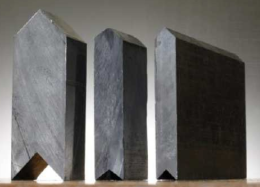
\includegraphics[width=\textwidth]{3DesignPrinciples/34BackgroundRejectionSystem/LeadBricks.png}  
    \caption{\label{subfig:LeadBricks}}
    \end{subfigure}
    \hfill
    \begin{subfigure}[b]{0.3\textwidth}
    \centering
    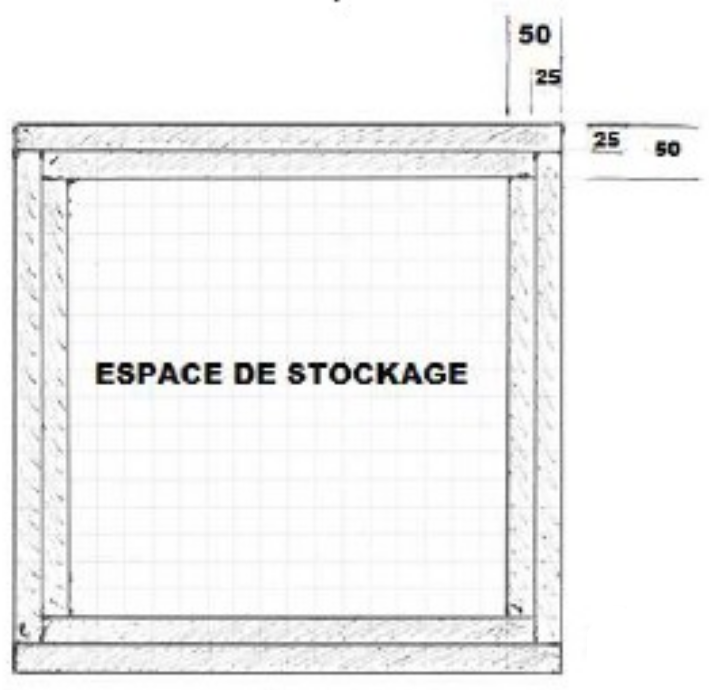
\includegraphics[width=\textwidth]{3DesignPrinciples/34BackgroundRejectionSystem/TwoLayers.png}  
    \caption{\label{subfig:TwoLayers}}
    \end{subfigure}
    \hfill
    \begin{subfigure}[b]{0.3\textwidth}
    \centering
    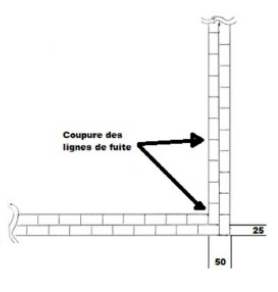
\includegraphics[width=\textwidth]{3DesignPrinciples/34BackgroundRejectionSystem/TwoLayers2.png}  
    \caption{\label{subfig:TwoLayers2}}
    \end{subfigure}
 \caption{a) Lead Bricks b) and c) Two layers for the lead bricks of the shield.}
 \label{fig:LeadBricksAndArrangement}
\end{figure}

A special aluminum structure, shown in Figure \ref{fig:AluminiumStructure}, was designed by mechanical engineering department of CENBG to support the total weight of $2.4$ tons of the lead bricks.

\begin{figure}
\centering
    \begin{subfigure}[b]{0.45\textwidth}
    \centering
    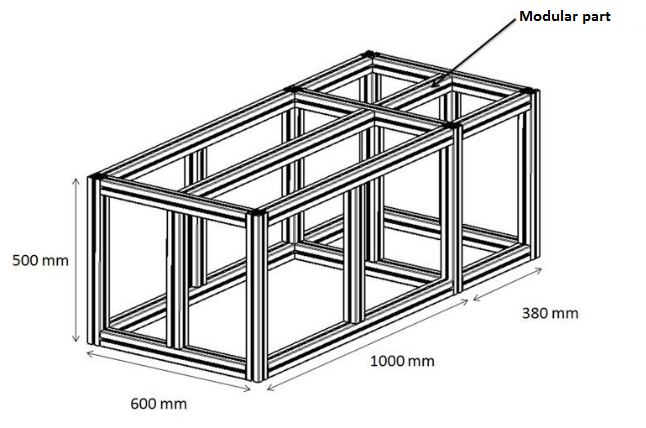
\includegraphics[width=\textwidth]{3DesignPrinciples/34BackgroundRejectionSystem/AluminiumStructureScheme.png}  
    \caption{\label{subfig:AluminiumStructureScheme}}
    \end{subfigure}
    \hfill
    \begin{subfigure}[b]{0.4\textwidth}
    \centering
    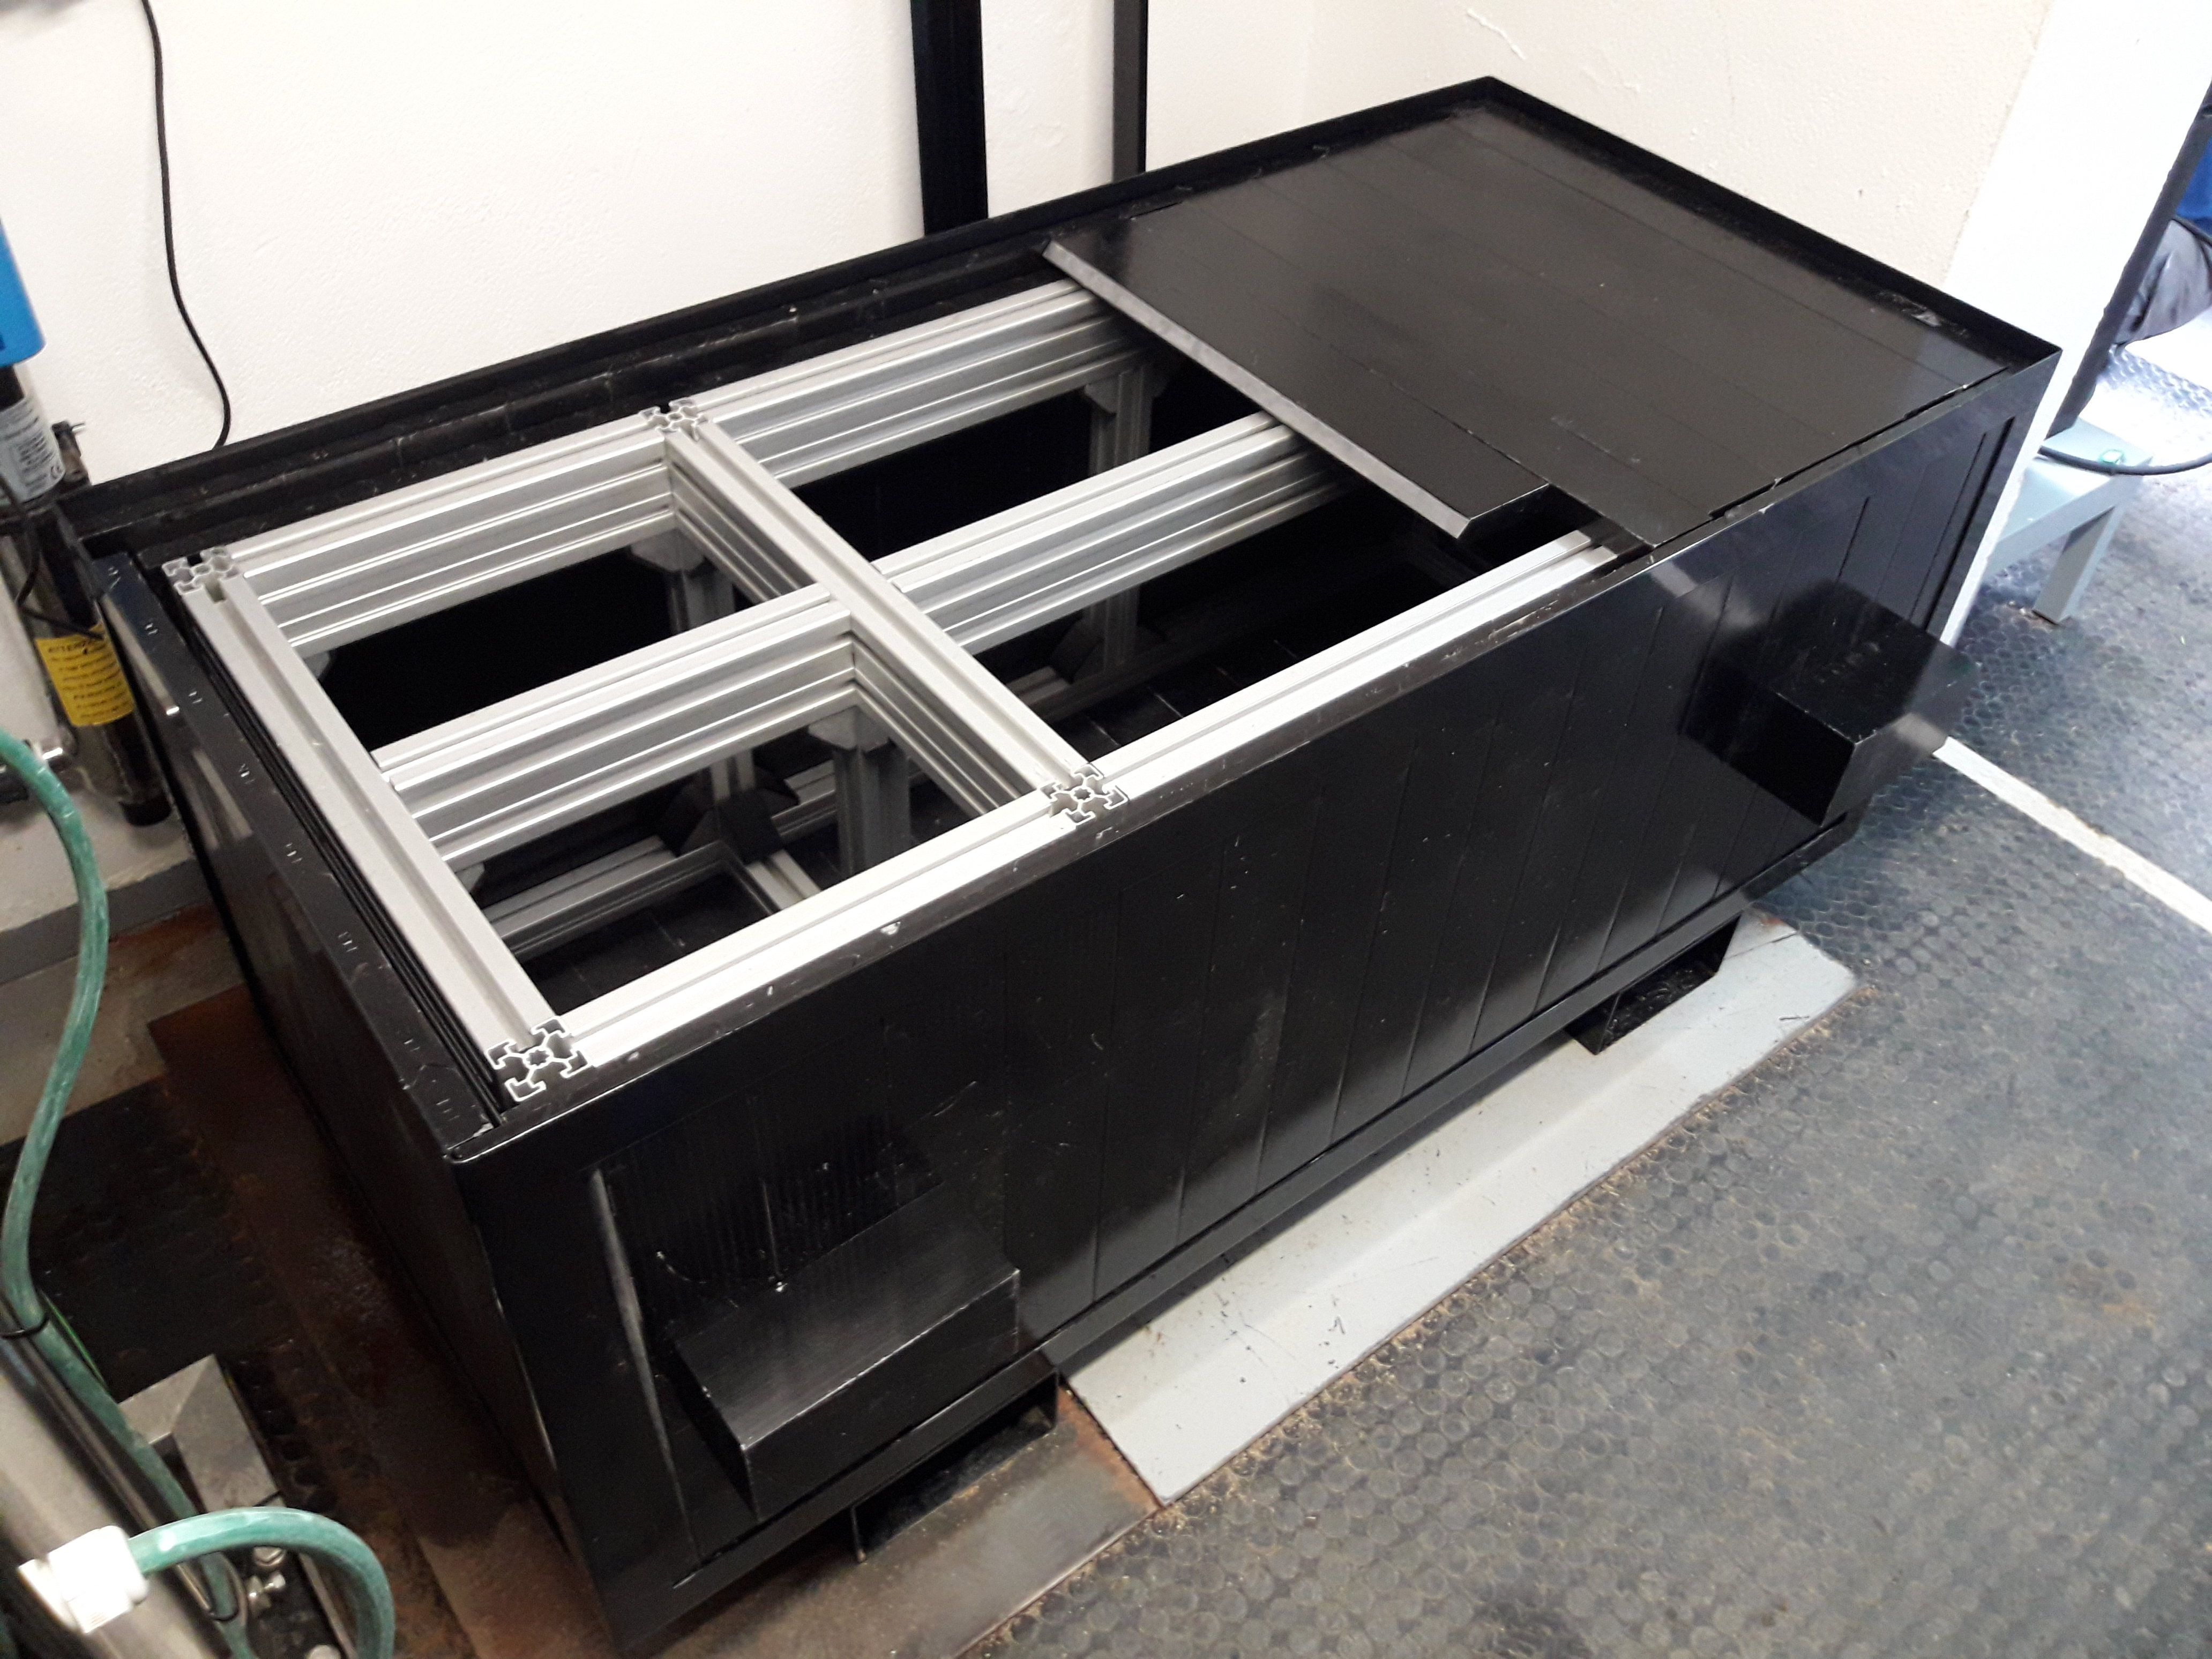
\includegraphics[width=\textwidth]{3DesignPrinciples/34BackgroundRejectionSystem/AluminiumStructure.jpg}  
    \caption{\label{subfig:AluminiumStructure}}
    \end{subfigure}
    \caption{a) Scheme of the aluminium structure of the shield; b) The lead shield partially mounted.}
 \label{fig:AluminiumStructure}
\end{figure}

The internal room of the lead shield is divided in two parts, as exhibited in Figure \ref{fig:AluminiumStructure}. The larger one has internal dimensions of $90.5 \times 41 \times 51~\cm^3$ and is used to place the TRITIUM detector. The smaller one, of dimensions of $33 \times 41 \times 51~\cm^3$, contains the Data Acquisition (DAQ) system of the detector. The external dimensions of the lead shield are $148 \times 60 \times 70~\cm^3$; its total weight is $2.5$ tons.